\subsection{Wheeled robot Kinematics}
\begin{wrapfigure}[7]{r}{0.2\columnwidth}
    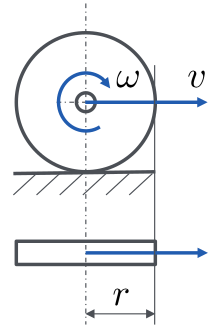
\includegraphics[width=0.2\columnwidth]{assets/wheel-constraints.png}
\end{wrapfigure}
\bi{Non-holonomic} systems \textbf{not integrable}, no inst. move in every direct.

\bi{Wheel constraints} $v_i = \omega_i r_i$

\begin{itemize}
    \item \textit{Driving straight} all $\vec{v}$ equal
    \item \textit{Turning} Wheel axis must intersect the \bi{Instant Centre of Rotation} (ICR),
          speeds: $v_i \div R_i = \Omega$ ($R_i$ dist. wheel-ICR, $\Omega$, vehicle body rotation rate)
\end{itemize}

\bi{Maneuverability}
\begin{itemize}
    \item Deg. of Mobility: $\delta_m = 3 - $\#constrained directions
    \item Deg. of Steerability: $\delta_s = $\#steerable wheels
    \item Deg. of Maneuverability: $\delta_M = \delta_m + \delta_s$
\end{itemize}

\bi{Wheel Configurations}

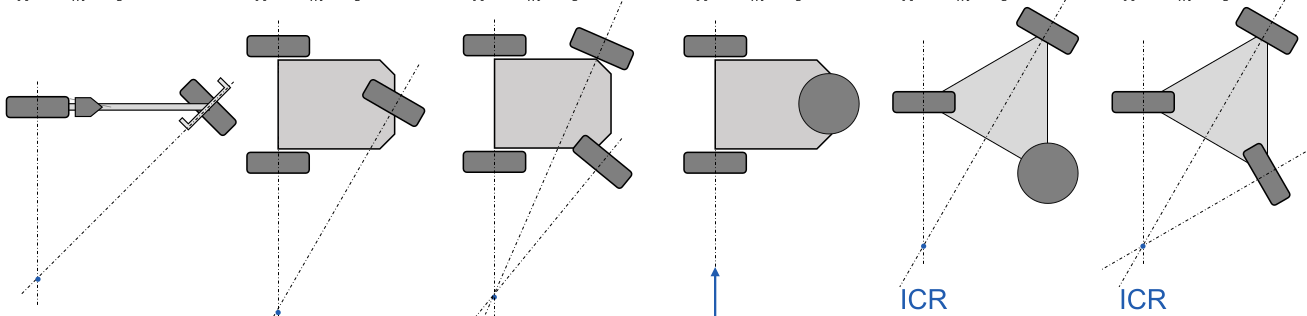
\includegraphics[width=1\columnwidth]{assets/wheel-config.png}

\begin{scriptsize}
    \begin{tabular}{llllll}
        Bicyle         & Tricycle       & Ackermann      & Diff. Drive    & Two-Steer      & Three-Steer    \\
        $\delta_m = 1$ & $\delta_m = 1$ & $\delta_m = 0$ & $\delta_m = 2$ & $\delta_m = 1$ & $\delta_m = 0$ \\
        $\delta_s = 1$ & $\delta_s = 1$ & $\delta_s = 2$ & $\delta_s = 0$ & $\delta_s = 2$ & $\delta_s = 3$ \\
        $\delta_M = 2$ & $\delta_M = 2$ & $\delta_M = 2$ & $\delta_M = 2$ & $\delta_M = 3$ & $\delta_M = 3$ \\
    \end{tabular}
\end{scriptsize}

\bi{Differential Drive Kinematics}

\bi{State vec} $\vec{x} = [x_1, x_2, \theta]^\top$,
\bi{Inputs} $\vec{u} = [\omega_l, \omega_r]^\top$, $r_r$ radius of right wheel, $w$ width of robot

\bi{Gen. eq. of Motion} $\dot{x}_1 = v\cos(\theta)$, $\dot{x}_2 = v\sin(\theta)$, $\dot{\theta} = \Omega$,
with $v = 0.5\cdot(\omega_l r_l + \omega_r + r_r)$, $\Omega = \frac{\omega_r r_r - \omega_l r_l}{w}$

\textit{Straight}: $v = \omega_l r_l = \omega_r r_r$, $\Omega = 0$, $D = v\Delta t$.\\
$\vec{b}_s = \begin{bmatrix}
        D \cos(\theta) \\
        D \sin(\theta) \\
        0
    \end{bmatrix}$
$\vec{b}_t = \begin{bmatrix}
    R(\sin(\Delta \theta + \theta) - \sin(\theta))\\
    -R(\cos(\Delta \theta + \theta) - \cos(\theta))\\
    \Delta \theta
\end{bmatrix}$

\textit{Turning}: $\Omega = (\omega_l r_l) / R_l\! =\! (\omega_r r_r) / R_r$, $R\! =\! v / \Omega$, $\Delta \theta\! =\! \Omega \Delta t$

\textbf{Discretized}: $\vec{x}_k = \vec{x}_{k - 1} b_i$ with $i \in \{s, t\}$. ($\int \ldots \dx \Delta t$)
